%%%%%%%%%%%%%%%%%%%%%%%%%%%%%%%%%%%%%%%%%%%%%%%%%%%%%%%%%%%%%%%%%%
% Sample template for MIT Junior Lab Student Written Summaries
% Available from http://web.mit.edu/8.13/www/Samplepaper/sample-paper.tex
%
% Last Updated August 30, 2011
%
% Adapted from the American Physical Societies REVTeK-4.1 Pages
% at http://publish.aps.org
%
% ADVICE TO STUDENTS: Each time you write a paper, start with this
% template and save under a new filename. If convenient, don't
%    erase unneeded lines, just comment them out.  Often, they
%    will be useful containers for information.
%
% Using pdflatex, images must be either PNG, GIF, JPEG or PDF.
%     Turn eps to pdf using epstopdf.
%%%%%%%%%%%%%%%%%%%%%%%%%%%%%%%%%%%%%%%%%%%%%%%%%%%%%%%%%%%%%%%%%%


%%%%%%%%%%%%%%%%%%%%%%%%%%%%%%%%%%%%%%%%%%%%%%%%%%%%%%%%%%%%%%%%%%
% PREAMBLE
% The preamble of a LaTeX document is the set of commands that precede
% the \begin{document} line.  It contains a \documentclass line
% to load the REVTeK-4.1 macro definitions and various \usepackage
% lines to load other macro packages.
%
% ADVICE TO STUDENTS: This preamble contains a suggested set of
% class options to generate a ``Junior Lab'' look and feel that
% facilitate quick review and feedback from one's peers, TA's
% and section instructors. Don't make substantial changes without
%     first consulting your section instructor.
%%%%%%%%%%%%%%%%%%%%%%%%%%%%%%%%%%%%%%%%%%%%%%%%%%%%%%%%%%%%%%%%%%

\documentclass[aps,twocolumn,secnumarabic,balancelastpage,amsmath,amssymb,nofootinbib]{revtex4}
%\documentclass[aps,twocolumn,secnumarabic,balancelastpage,amsmath,amssymb,nofootinbib]{revtex4-1}
\pdfpagewidth 8.5in
\pdfpageheight 11in

\usepackage{lgrind} % convert program listings to a form includable in a LaTeX document
\usepackage{chapterbib} % allows a bibliography for each chapter(each labguide has it's own)
\usepackage{color} % produces boxes or entire pages with coloredbackgrounds
\usepackage{graphics}      % standard graphics specifications
\usepackage[pdftex]{graphicx} % alternative graphics specifications
\usepackage{longtable}     % helps with long table options
\usepackage{epsf} % old package handles encapsulated post scriptissues
\usepackage{bm}            % special 'bold-math' package
%\usepackage{asymptote} % For typesetting of mathematical illustrations
\usepackage{thumbpdf}
\usepackage[colorlinks=true]{hyperref} % this package should be added after all others
% use as follows: \url{http://web.mit.edu/8.13}
\usepackage{multirow}
\usepackage{subfigure}

% Define a useful new command for writing units
\newcommand{\cd}{$\cdot$}

%
% And now, begin the document...
%

\begin{document}
\title{Zenith Angle Distribution of Cosmic Ray Muons}
\author{Jay M.\ Lawhorn}
\email{klawhorn@mit.edu}
\date{\today}
\affiliation{MIT Department of Physics}

\begin{abstract}
The zenith angle distribution of cosmic ray muons is investigated using two scintillating paddles to make a detector with sensitivity to the interaction position and therefore angular distribution. The effective speed of light in the scintillator is measured as $(7.6\pm0.5)$ cm/ns. A monte carlo simulation of the physical detector using measurements of the detector response to a radium-226 source at various points along the detector indicates that the acquired data is consistent with the predicted $\cos^{2}{\theta}$ distribution, but cannot rule out a flat angular distribution. 
\end{abstract}

\maketitle

\section{Introduction}

The upper atmosphere is continuously bombarded by energetic electrons, hadrons, and light nuclei from extraterrestrial sources~\cite{pdg}. Interactions between this cosmic radiation and the upper atmosphere produce secondary showers that contain unstable particles. Muons are primary component of cosmic rays at sea level, and were first observed in cosmic radiation. They have a lifetime of 2.2 $\mu$s, which is ample time for the highly relativistic cosmics to traverse the atmosphere as well as a significant distance below ground.

The survival of muons produced in the upper atmosphere at sea level was an early confirmation of special relativity because without time dilation a much smaller rate is expected at sea level based on high altitude measurements and classical mechanics. 

The predicted zenith angle, $\theta$, distribution of incident cosmic ray muons is dependent on the muon energy distribution, detector altitude, and other factors~\cite{pdg}. However, it is commonly approximated as 
\begin{equation}
I(\theta) = I_0 \cos^{2}{\theta}
\end{equation}
where $I_0$ is the vertical intensity of incident muons~\cite{kuo}. This experiment aims to validate this approximation. 

\section{Apparatus}

\begin{figure}[htb]
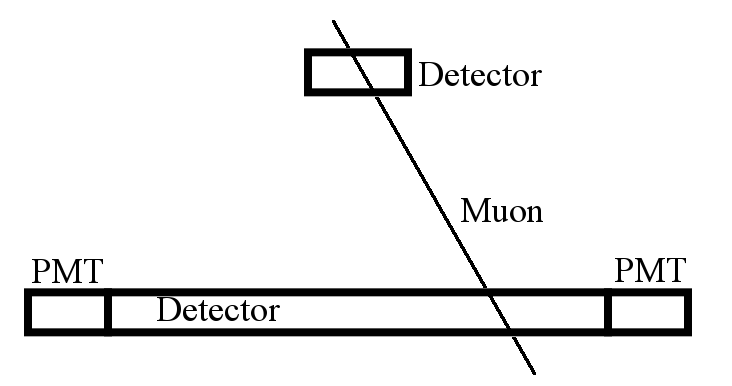
\includegraphics[width=8cm]{paddles.png}
\caption{Detector geometry. The lower scintillating detector has two PMTs viewing each short end of the detector, while the upper scintillating detector has a single PMT viewing it. Muon tracks are reconstructed based on the pulse arrival times in the lower PMTs and requiring a coincident signal in the upper detector. }
\label{paddles}
\end{figure}

The detectors, shown in Figure \ref{paddles}, consists of two scintillating paddles separated by 46.6 cm. The lower paddle consists of 188 cm by 10 cm of scintillating plastic. Both 10 cm edges are attached to a photomultipler tube (PMT) by a light guide. The two PMTs of the lower paddle are operated at -2.03 kV. The upper paddle is 11.3 cm by 11.7 cm of scintillator with a single PMT attached to an 11.3 cm edge operated at -1.90 kV. The other 11.3 cm edge is aligned with the long edge of the bottom paddle. The left edge of the upper paddle is 90.5 cm away from the left edge of the bottom paddle. The detector geometry used is sensitive to angles below 65$^o$. 


All scintillating paddles and PMTs are wrapped in a light-tight plastic, and no differences in baseline PMT output level or rate were observed when the overhead lights in the lab were turned off, suggesting that the apparatus does not suffer from significant light leaks. 

The subsequent data acquisition chain is shown in Figure \ref{chain}. An equal length of cable, approximately 4 m, connects each PMT to a discriminator, which outputs a negative square pulse when a the PMT signal exceeds a certain threshold. The two lower PMT thresholds are set at 6 mV, while the upper PMT threshold is 10 mV. The output of the three discriminators is split, and sent to a coincidence unit which outputs a negative square pulse when all three discriminators fire within a short window. 

\begin{figure}[htb]
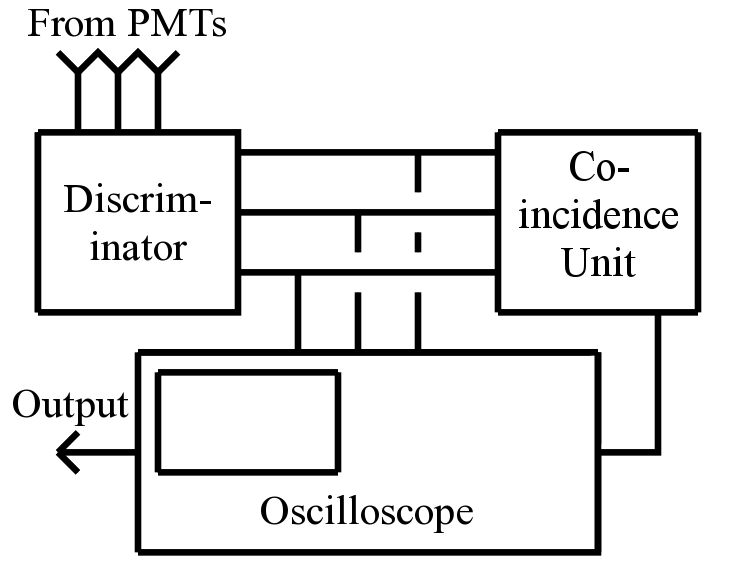
\includegraphics[width=8cm]{chain.png}
\caption{Signal chain after PMT output. The three signals are passed through a discriminator, which outputs logic pulses to a coincidence unit. The coincidence unit triggers an associated oscilloscope which records the timing differences between the various discriminator pulses. }
\label{chain}
\end{figure}

Both the coincidence output and the other half of the discriminator outputs are sent to an oscilloscope that triggers on the falling edge of the coincidence unit output. The discriminator outputs are each delayed by approximately 4 m of cable such that the scope sees the discriminator outputs at approximately the same time as the coincidence unit signal. 

The Rigol oscilloscope is controlled using its native scripting interface, PyVISA, and Python \cite{teq,pyvisa,python}. Time intervals between each rising pulse within a 60 ns window centered on the trigger pulse are measured and saved. The oscilloscope has 0.1 ns resolution, but all differences less than 1 ns are reported as ``$<$1ns", which is subsequently converted to a 0 ns measurement.

Six total time differences are measured: $\Delta T_{LC}$, between the left PMT pulse edge and coincidence pulse edge; $\Delta T_{RC}$, between the right PMT pulse edge and coincidence; $\Delta T_{TC}$, between the top PMT pulse edge and coincidence; $\Delta T_{LR}$, between left PMT and right PMT; $\Delta T_{LT}$, between left PMT and top PMT; $\Delta T_{RT}$, between right PMT and top PMT.

Light from the primary interaction of the detected particle and scintillator travels at the speed of light in the medium, which must be established. The difference in arrival times of a signal at the two ends of the long scintillator paddle are used to reconstruct the interaction position along the long axis of the scintillator. 

\section{Scintillator Characterization}

The speed of light in the medium is measured using a small radium-226 probe. From a point a distance $x$ along the lower detector measured from the left PMT, the time delay is $t_L = x/v_{eff}$, where $v_{eff}$ is the effective speed of light in the scintillator. Similarly, the time delay in the right PMT is $t_R = (L-x)/v_{eff}$, where $L$ is 188 cm. 

Combining these two equations, the position $x$ is given by 
\begin{equation}
x=\frac{v_{eff}}{2}\Delta t_{LR} + L. 
\end{equation}

The radium-226 probe is placed along the center line at ten different points along the lower detector ranging from the left edge to the right edge in steps of approximately 20 cm. The full list of probe locations is summarized in Table~\ref{data}, as well as the number of events at each location. 

\begin{table}[hb]
\caption{\label{data} Summary of acquired data. The third column gives the number of events that pass the cleaning criteria described in the text for each data taking condition.}
\begin{tabular}{|c|c|c|}
\hline
Operating Condition & Total Events & Cleaned Events \\
\hline
Source, 0 cm & 200 & 170 \\
\hline
Source, 20 cm & 100 & 95 \\
\hline
Source, 40 cm & 100 & 93 \\
\hline
Source, 60 cm & 100 & 89 \\
\hline
Source, 80 cm & 100 & 93 \\
\hline
Source, 100 cm & 200 & 178 \\
\hline
Source, 120 cm & 200 & 163 \\
\hline
Source, 140 cm & 200 & 162 \\
\hline
Source, 160 cm & 200 & 190 \\
\hline
Source, 188 cm & 200 & 193 \\
\hline
No source & 1888 & 1875 \\
\hline
\end{tabular}
\end{table}

Coincident events in the two lower PMTs are required for this setup, but no coincidence with the upper paddle is required. One hundred events at each probe location are acquired, and an additional one hundred events are acquired for approximately half of the locations based on the observed complexity of the time difference distribution.

The arrival time in the left and right PMTs are taken as $\Delta t_{LC}$ and $\Delta t_{RC}$ respectively. Events where either time difference is recorded as ``9E37" are discarded. For events where one or the other time difference is recorded as 0 ns because of the oscilloscope's 1 ns measurement threshold, an equivalent sum of time differences are used. For example, if $\Delta t_{LC}$ is recorded as 0 ns, it is replaced by $\Delta t_{LR}+\Delta t_{RC}$.

Distributions of the value $\Delta t_{LR} = \Delta t_{LC} - \Delta t_{RC}$ for each source location are shown in Figure~\ref{dists}. The time delay is measured in this way because the direct measurement of the time difference between the two arrival times was often recorded as 0 ns and the alternate calculation yields a more precise value that is still always smaller than the reported 1 ns. 

For each dataset, the mean time delay is computed using the binned data, weighted by the statistical uncertainty on each bin count. The mode time delay is also computed for each data set, and the difference between the computed mean and mode is taken as a systematic uncertainty on the time delay measurement. The mean time delay was chosen as the nominal value because the mode is more sensitive to statistical fluctuations and choice of bin width. However, the two are expected to be similar for a centered distribution like the time delay. The total uncertainty on each measured time delay is taken to be the sum in quadrature of the statistical uncertainty from the weighted mean calculation and the systematic uncertainty from the difference between mean and mode values. 

\begin{figure}[htb]
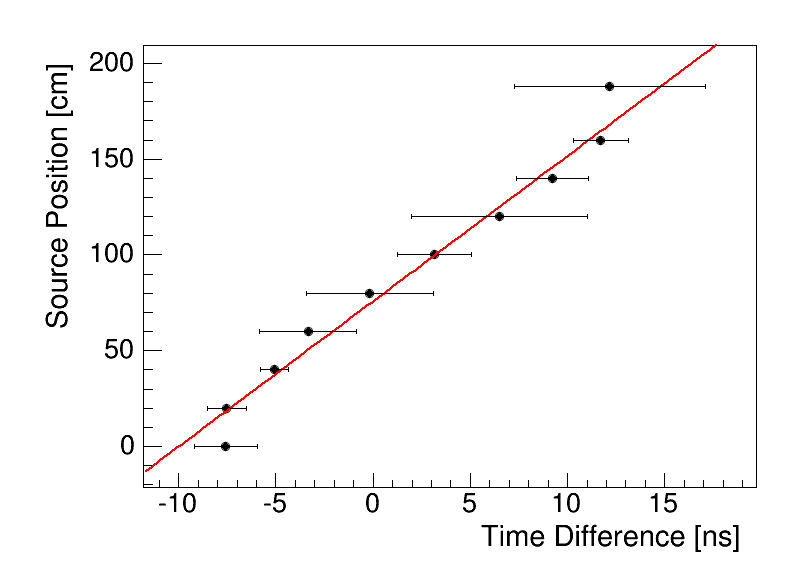
\includegraphics[width=8cm]{rad_vel.png}
\caption{Source position as a function of measured time difference between the two PMT signals. Note that the curve is not centered at 0, indicating that the total delay in the signal chain after each PMT is not exactly equal.}
\label{vel}
\end{figure}

The measured results are shown in Figure~\ref{vel} with a fit to a first degree polynomial. The speed of light in the scintillator is measured to be $(7.6\pm0.5)$ cm/ns. This is much lower than the predicted value based on the index of refraction of the medium, 20 cm/ns, because the majority of the photons reaching the PMT do not travel along a straight path from initial scintillation point to the PMT, instead being internally reflected several times along the way. 

The measured velocity curve appears to be consistent with a linear relation over much of the detector, with some deviation near each end. This is expected because light extinction and energy loss become most relevant at long distances traveled, which occur when the primary interaction point is maximally separated from one PMT or the other by falling at the opposite end of the detector. 

\section{Muons}

To observe muon events, the radium-226 source is removed, and coincidence is required between all three PMTs. Data is acquired over 96 hours, for a total sample of 1888 events. A cleaning process identical to the one described above for the radium-226 data, with the addition of similar requirements on the top PMT pulses, is used. Only 13 events are discarded for a final sample size of 1875 events. 

A monte carlo technique is employed to simulate muon events in our detector. The TRandom3 class in ROOT~\cite{root} with a randomly initialized seed was used for all random number generation. Random values representing the point of interaction on the upper paddle are generated, assuming an isotropic distribution.

Random values for each muon's direction in ($\theta$, $\phi$) are also generated based on three different underlying distributions. The first is the literature standard $\cos^2{\theta}$ distribution that is isotropic in $\phi$~\cite{kuo}. A distribution that is isotropic in both $\theta$ and $\phi$ is also considered, as well as a very non-physical scenario corresponding to a collimated muon source at $\theta=\pi/4$ and $\phi=0$. The last is included to demonstrate the rejection power of the following analysis. 

The predicted primary interaction point distributions for each of the three considered angular distributions are shown in Figure~\ref{bah}. The flat angular distribution and the nominal distribution result in fairly similar distributions, with the flat distribution resulting in a slightly wider distribution along the long axis. The collimated muon source scenario results in a much different distribution than the other two. 

\begin{figure}[htb]
\centering
\subfigure{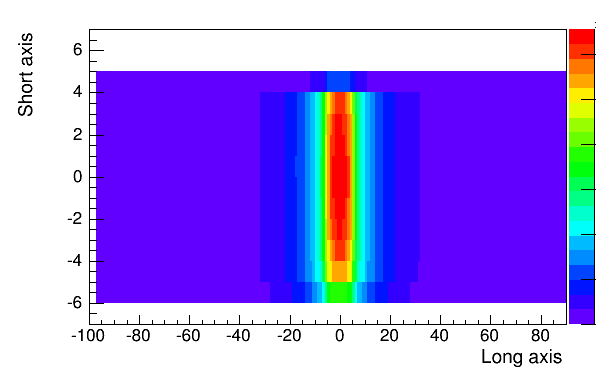
\includegraphics[width=6cm]{nominal_dist.png}} 
\subfigure{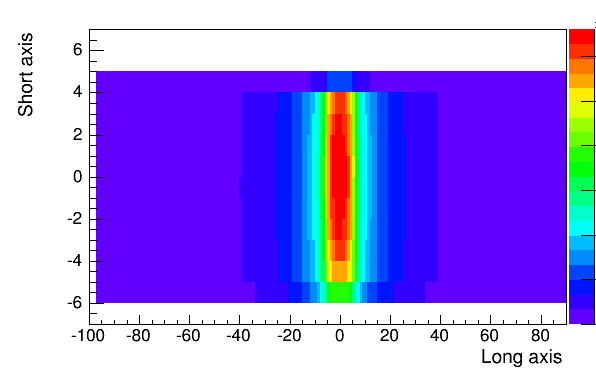
\includegraphics[width=6cm]{flat_dist.png}}
\subfigure{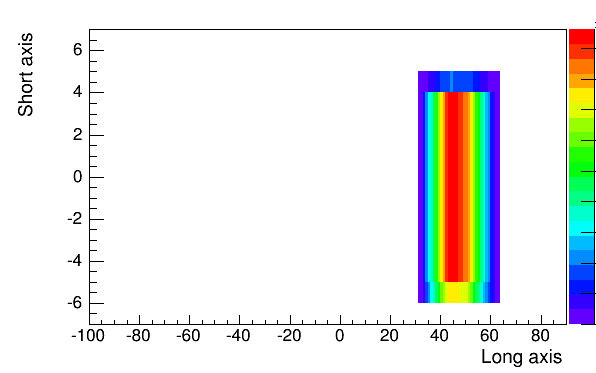
\includegraphics[width=6cm]{fuck_dist.png}}
\caption{\label{bah} Predicted primary interaction point distributions for the (top) nominal distribution, (middle) flat distribution, and (bottom) collimated source distribution. Note that the flat distribution results in a wider distribution along the long axis than the nominal distribution.  }
\end{figure}

One billion events for each underlying distribution are generated, and projected into the plane of the lower paddle. The acceptance of the lower paddle is taken into account by discarding events that fall outside the measured detector geometry as described above. 

Instead of attempting to simulate the scintillator and PMT response to incident muons from first principles, the radium-226 data is used to create a data-driven estimate of the detector response for a given primary interaction point. The detector is split into ten regions centered on each of the source locations, and a time difference is chosen at random from the measured time difference distribution at the source location corresponding to the region containing the simulated event's primary interaction point. 

The collected data is separated into 20 bins ranging from from time differences of -40 to 40 ns. The simulated distribution for each underlying geometry is fit to the data with a single parameter describing the normalization. The value of $\chi$ for each bin is calculated where
\begin{equation}
\chi = \frac{n_{obs}-n_{exp}}{\sqrt{n_{exp}}}
\end{equation}
where $n_{obs}$ is the number of events observed in a given bin and $n_{exp}$ is the number of events expected in a given bin. 

The fitted distributions and $\chi$ values are shown in Figure~\ref{results}. The nominal and flat angular distributions result in extremely similar time difference distributions and calculated $\chi$ values, indicating that they are comparably compatible with the obtained data. However, as expected, the collimated source scenario results in an incompatible time difference distribution and much larger $\chi$ values. This demonstrates that the experimental setup has some ability to differentiate various underlying cosmic ray muon distributions, but not enough to differentiate the nominal distribution from a flat distribution. 

The experimental results are therefore compatible with the nominal $\cos^{2}{\theta}$ distribution, but cannot rule out a flat angular distribution. However, the non-physical collimated off-axis source model can be ruled out, demonstrating that the setup has some sensitivity to the underlying model.

A conclusive study using the same experimental apparatus might be possible, but it would require much better timing resolution and position reconstruction. It is likely that including information about the PMT pulse shape, most importantly the pulse height, could provide this additional information. The pulse height decreases with increased distance traveled through the scintillator because of energy loss in the material, so that information could help differentiate a multiply reflected photon from a photon that is not reflected at all when combined with the measured arrival time. 

A study of the pulse height effect on the slew time delay of the discriminator output would also improve the results. Slew time delays are most prominent for small pulses, which take a longer fraction of the PMT response time to reach the discriminator threshold, thus introducing an additional delay in the measured arrival time. This analysis assumes that the measured time difference distributions from the radium-226 data appropriately corrects for these effects, but a study of pulse height and slew time would likely yield a more physically descriptive model. 

\begin{thebibliography}{9}

\bibitem{pdg}
J. Beringer et al. (Particle Data Group), \emph{Cosmic Rays}, Phys. Rev. D86, 0100001 (2012).

\bibitem{kuo}
Y. Kuo, \emph{Determination of the Angular Distribution of Cosmic Rays at Sea Level}. Senior Thesis, Massachusetts Institute of Technology (2010). 

\bibitem{teq}
RIGOL Technologies, \emph{Programming Guide: DS1000B Series Digital Oscilloscope}. PGA04108-1110 (2011). See \url{http://www.tequipment.net/assets/1/26/Documents/Rigol/DS1064B/ds1064b_doc_1.pdf}. 

\bibitem{pyvisa}
H. Grecco, et al. (PyVISA authors). Obtained from \url{https://github.com/hgrecco/pyvisa}. 

\bibitem{python}
G. van Rossum and F.L. Drake (eds), Python Reference Manual, (2014). See \url{http://www.python.org}.  

\bibitem{root}
R. Brun and F. Rademakers, \emph{ROOT - An Object Oriented Data Analysis Framework}, Proceedings AIHENP'96 Workshop, Lausanne, Sep. 1996, Nucl. Inst. \& Meth. in Phys. Res. A 389 (1997) 81-86. See also \url{http://root.cern.ch/}.

\end{thebibliography}

\clearpage

\begin{figure*}
\centering
\subfigure{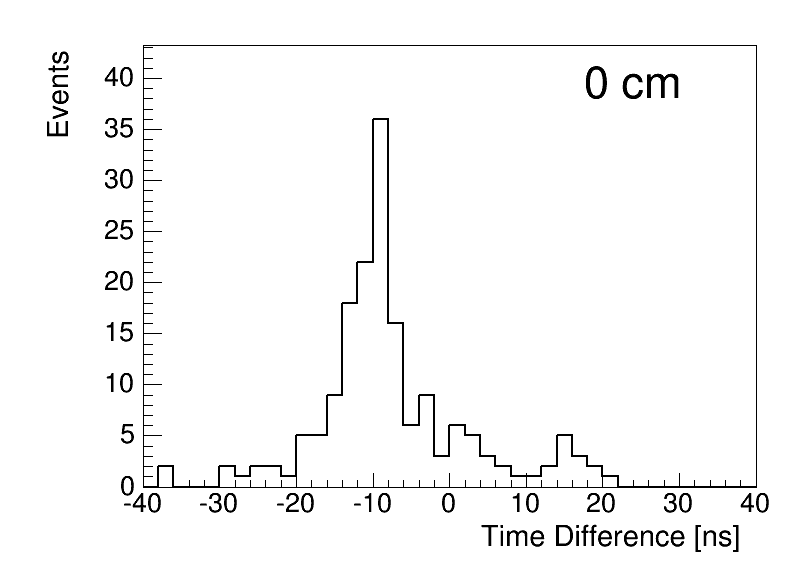
\includegraphics[width=6cm]{rad_diff0.png}} 
\subfigure{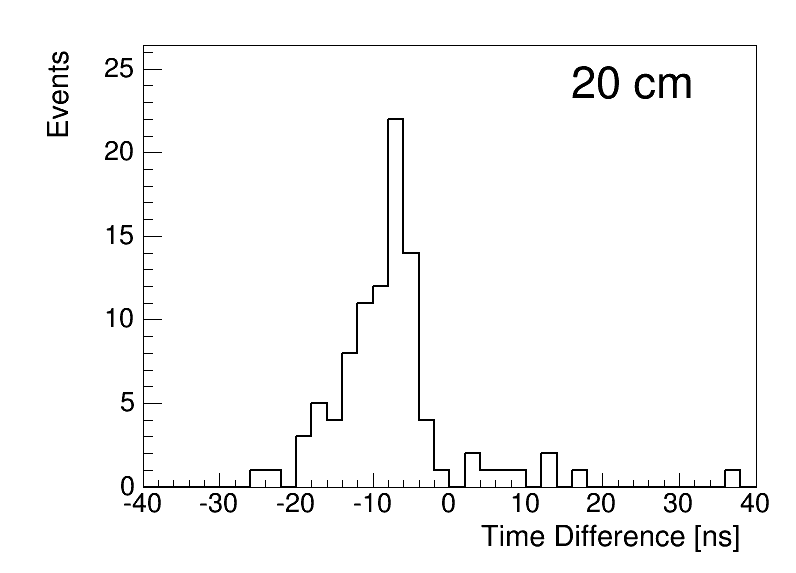
\includegraphics[width=6cm]{rad_diff1.png}}
\subfigure{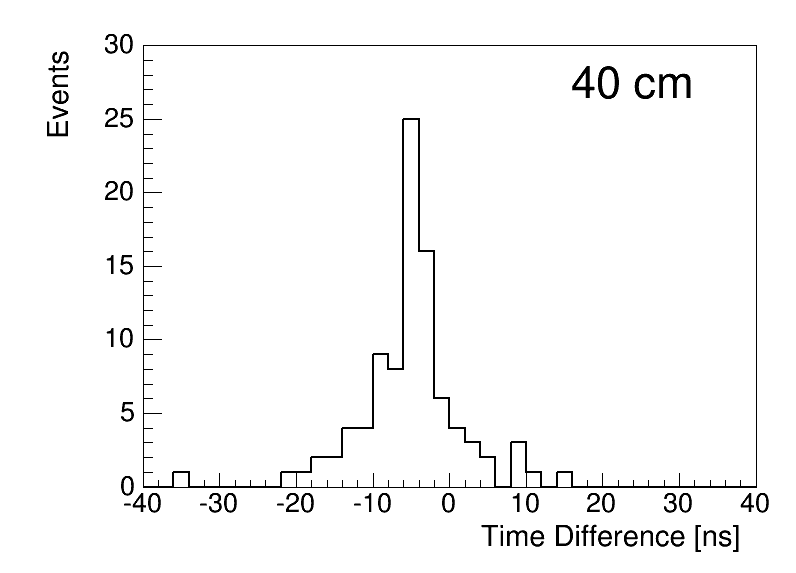
\includegraphics[width=6cm]{rad_diff2.png}}
\subfigure{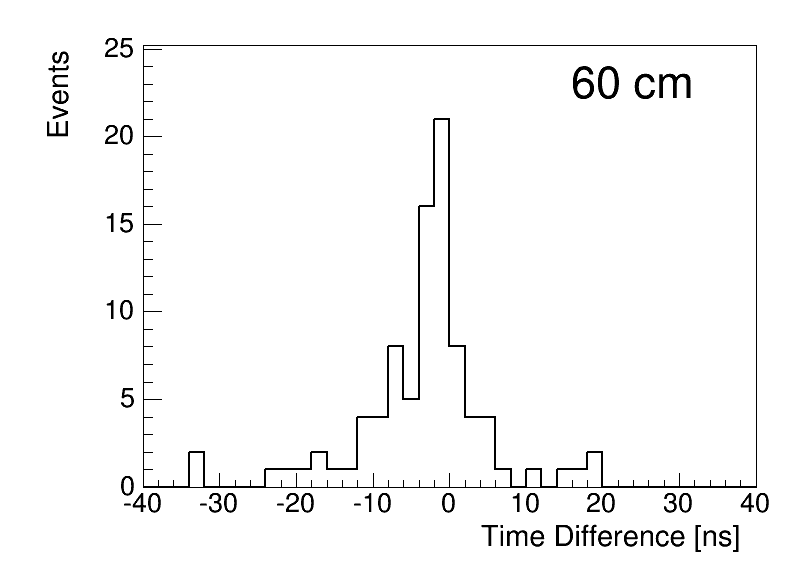
\includegraphics[width=6cm]{rad_diff3.png}}
\subfigure{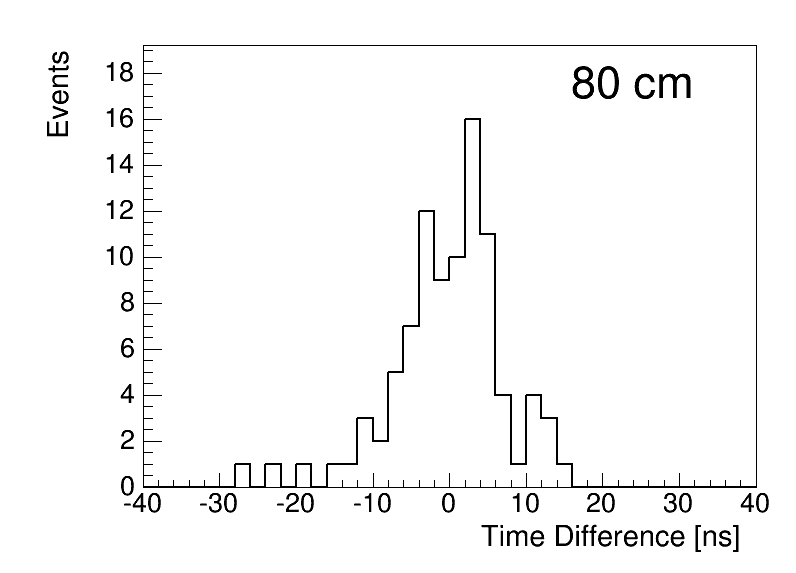
\includegraphics[width=6cm]{rad_diff4.png}}
\subfigure{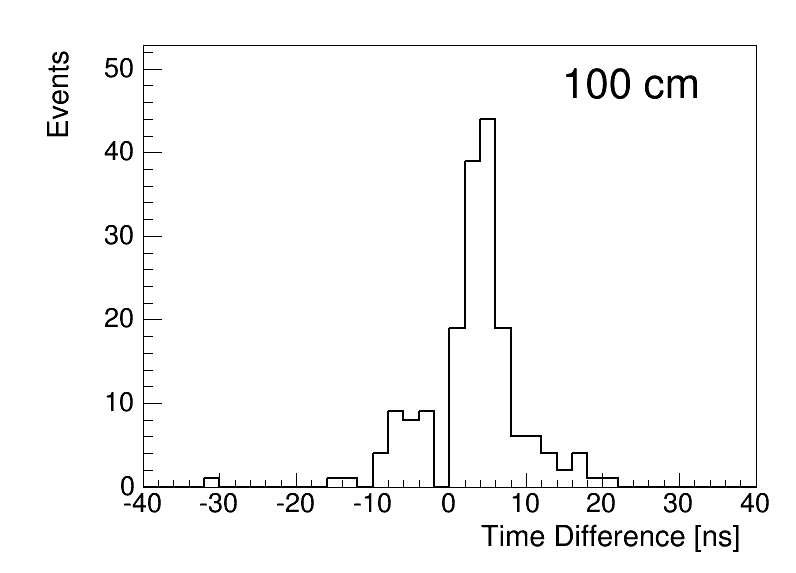
\includegraphics[width=6cm]{rad_diff5.png}}
\subfigure{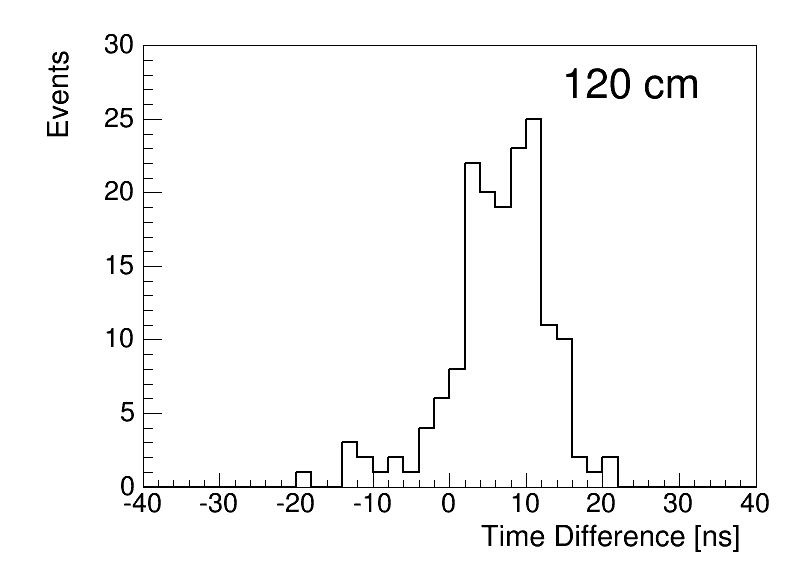
\includegraphics[width=6cm]{rad_diff6.png}}
\subfigure{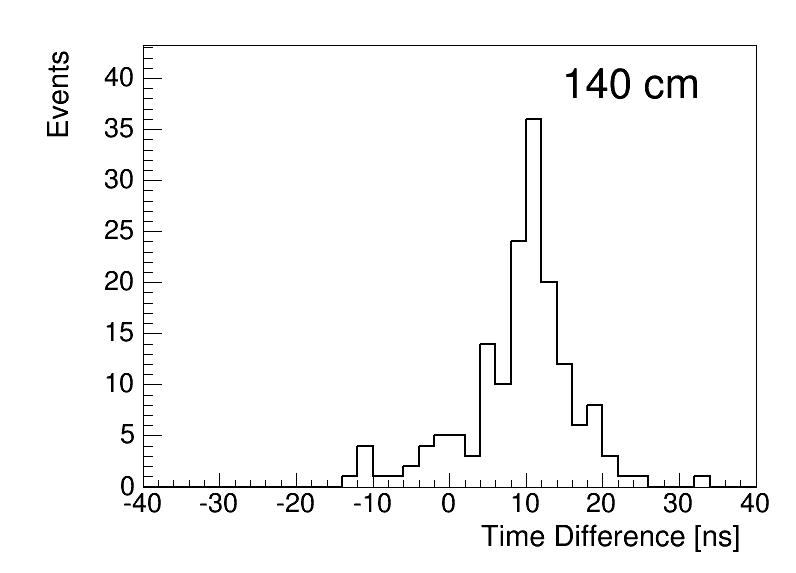
\includegraphics[width=6cm]{rad_diff7.png}}
\subfigure{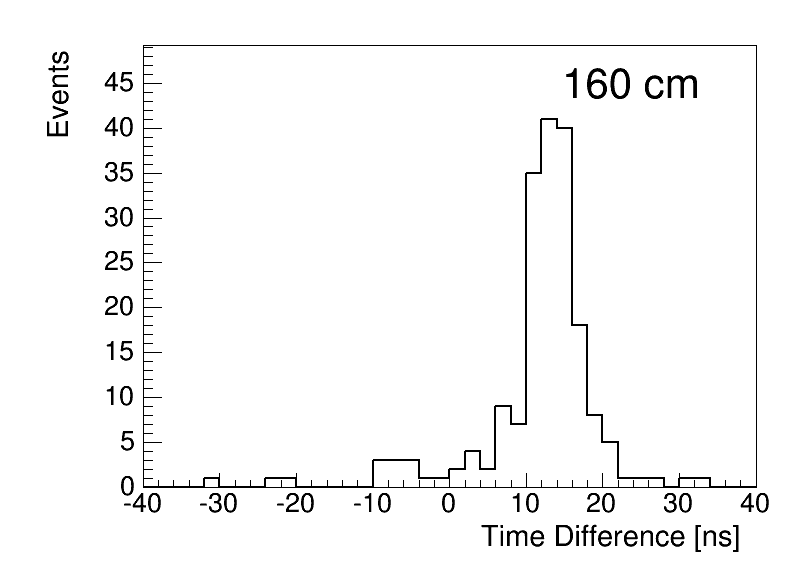
\includegraphics[width=6cm]{rad_diff8.png}}
\subfigure{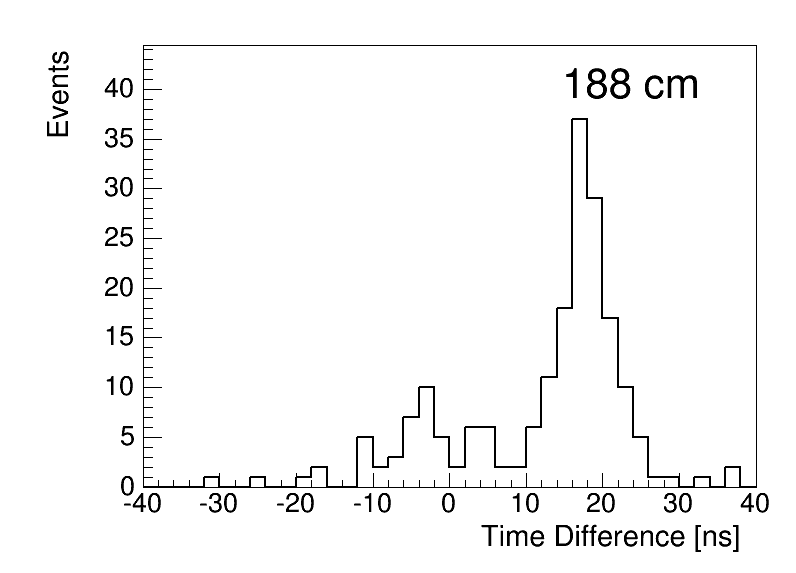
\includegraphics[width=6cm]{rad_diff9.png}}
\caption{\label{dists} Measured time difference distributions for each radium-226 location along the lower scintillating paddle. The location of the source is listed at upper right of each plot. }
\end{figure*}

\begin{figure*}[htb]
\centering
\subfigure{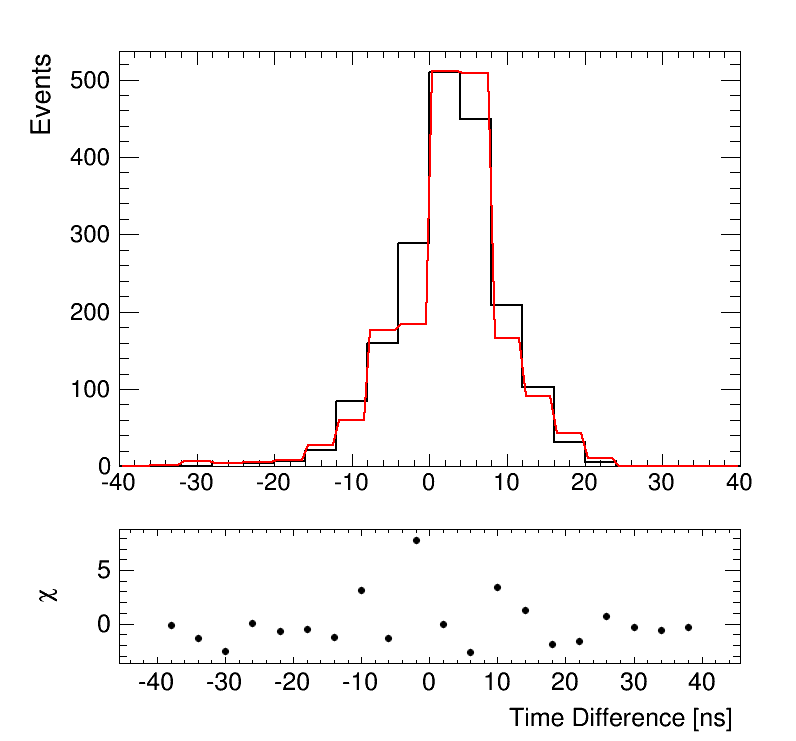
\includegraphics[width=7cm]{nominal.png}} 
\subfigure{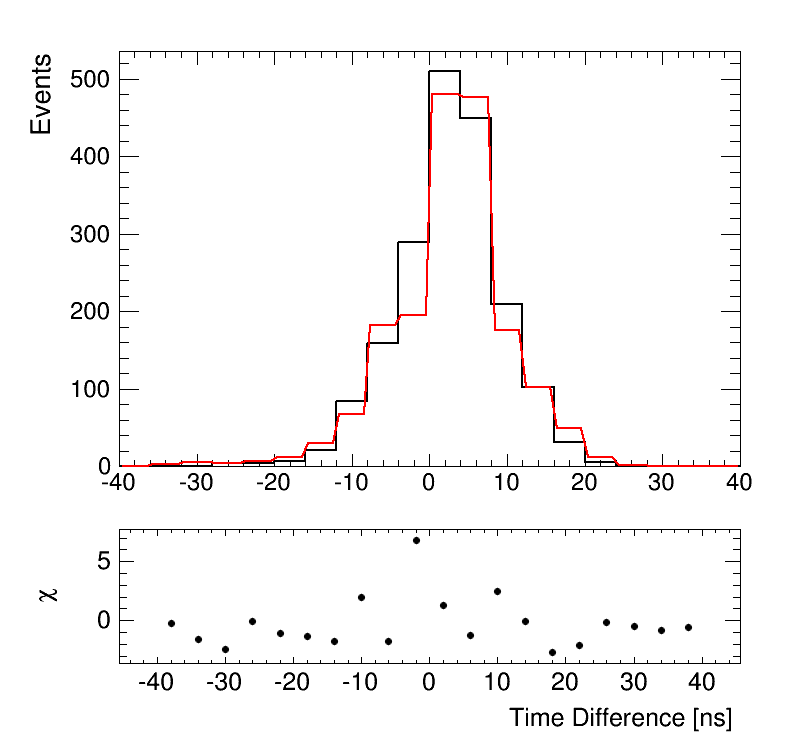
\includegraphics[width=7cm]{flat.png}}
\subfigure{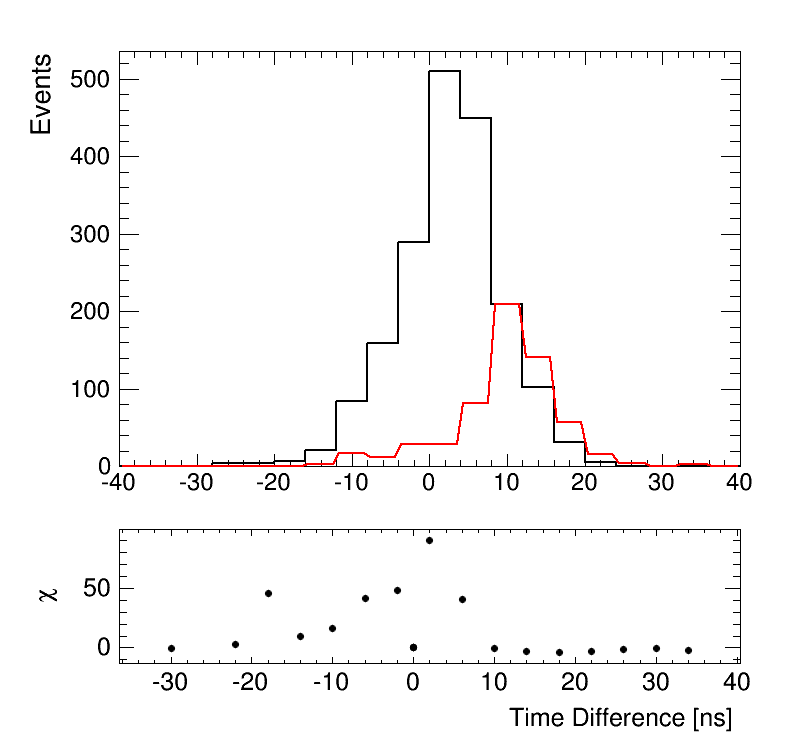
\includegraphics[width=7cm]{fuck.png}}
\caption{\label{results} Fits of monte carlo (red) distributions to obtained data (black) for the (upper left) nominal angular distribution, (upper right) flat angular distribution, and (bottom) collimated source geometry. The $\chi$ value for each bin calculated as described in the text is plotted below the distributions. }
\end{figure*}

\end{document}
